\chapter{Język ViuAct i jego kompilator -- implementacja}
\label{viuact_impl}
\label{jezyk_viuact_i_jego_kompilator}

Pierwszą częścią naszej pracy jest zaprojektowanie wysokopoziomowego języka programowania i opracowanie jego
implementacji. Z uwagi na to, że platforma uruchomieniowa, którą wykorzystujemy (czyli Viua VM) jest maszyną
wirtualną wykonującą programy w postaci \emph{bytecode} wybranym sposobem implementacji języka jest
kompilator - program tłumaczący kod źródłowy w jednym języku na kod źródłowy w innym języku przy jednoczesnym
zachowaniu zachowania programu. W przypadku naszej pracy językiem źródłowym jest język Viuact (dokładniej
opisany w rozdziale \ref{specyfikacja_jezyka_viuact}.~\nameref{specyfikacja_jezyka_viuact} na stronie
\pageref{specyfikacja_jezyka_viuact}), a językiem docelowym język assemblera Viua VM.

\section{Architektura}

\subsection{Użyte wzorce projektowe -- Sposób konstrukcji kompilatora}

\begin{figure}[!htp]
    \centering
    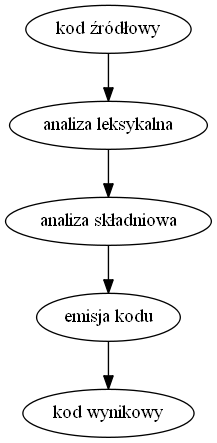
\includegraphics[width=5cm]{basic-compiler-flow}
    \caption{Podstawowy schemat budowy kompilatora}
    \label{basic_compiler_flow}
\end{figure}

Na rysunku \ref{basic_compiler_flow} przedstawiony jest uproszczony schemat budowy kompilatora.
W kompilatorach ''produkcyjnych'' (np. GCC, Clang, czy ICC) tych faz jest więcej -- przede wszystkim etap
emisji kodu jest dużo bardziej rozbudowany, oraz dochodzą etapy analizy semantycznej (czy program ma sens) czy
optymalizacji (prób takiego przekształcenia kodu programu żeby przy zachowaniu znaczenia działał wydajniej).

Kompilator języka ViuAct dostarczany jako element tej pracy inżynierskiej jest pozbawiony etapów
analizy semantycznej oraz optymalizacji. Analiza semantyczna (oraz weryfikacja typów i wykrywanie błędów na
etapie kompilacji) jest oddelegowana do assemblera dostarczanego przez platformę. Optymalizacja jest
całkowicie pominięta gdyż jest to temat niezwykle rozległy; implementacja i doszlifowanie algorytmów
optymalizujących kod jest sama w sobie materiałem wystarczającym na napisanie osobnej pracy inżynierskiej.

Architektura kompilatora języka ViuAct jest dokładniej opisana w rozdziale
\ref{architektura_kompilatora_viuact} (\nameref{architektura_kompilatora_viuact}) na
stronie \pageref{architektura_kompilatora_viuact}.
Sposób działania kompilatora jest opisany w rozdziale \ref{opis_etapow_kompilacji}
(\nameref{opis_etapow_kompilacji}) na stronie \pageref{opis_etapow_kompilacji}.
Omówienie interakcji kompilatora języka ViuAct z narzędziami dostarczanymi przez platformę Viua VM znajduje
się w rozdziale \ref{lang_architektura_systemu} (\nameref{lang_architektura_systemu}) na stronie
\pageref{lang_architektura_systemu}.

Oprócz kompilatora (rozdział \ref{opis_kompilatora} na stronie \pageref{opis_kompilatora}) dostarczany jest
również ''program łączący'' (rozdział \ref{opis_linkera} na stronie \pageref{opis_linkera}) dokonujący
automatycznego połączenia wymaganych modułów w gotowy plik wykonywalny.

\subsection{Architektura systemu}
\label{lang_architektura_systemu}

Rysunek \ref{schemat_interakcji_viuact_z_viuavm} (''\nameref{schemat_interakcji_viuact_z_viuavm}'') prezentuje
schemat interakcji jakie zachodzą w całym systemie od momentu wczytania pliku źródłowego przez kompilator do
uruchomienia programu przez jądro Viua VM.

Ostatnią fazą jaką zajmuje się kompilator języka ViuAct dostarczany jako element tej pracy inżynierskiej jest
emisja kodu (''Assembly code emission''), której wynikiem jest plik z kodem źródłowym w języku assemblera Viua
VM (''\texttt{hello\_world.asm}'' na rysunku \ref{schemat_interakcji_viuact_z_viuavm}).
Rozdział \ref{architektura_kompilatora_viuact} (\nameref{architektura_kompilatora_viuact}) dokładniej opisuje
działanie samego kompilatora.

\begin{figure}[!htp]
    \centering
    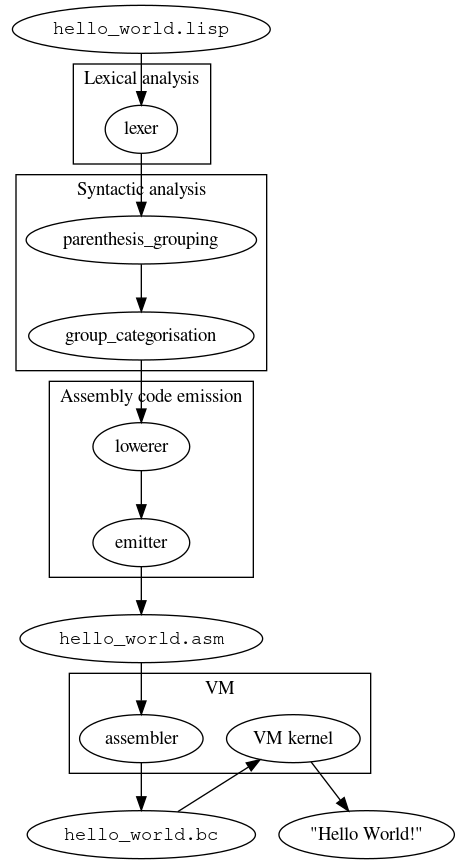
\includegraphics[width=9cm]{viuact-pipeline}
    \caption{Interakcje: od pliku źródłowego do działającego programu}
    \label{schemat_interakcji_viuact_z_viuavm}
\end{figure}

Zakres pracy inżynierskiej obejmuje wygenerowanie pliku zawierającego poprawny kod w języku
assemblera Viua VM oraz plików pomocniczych (zadanie kompilatora), oraz takim pokierowaniu
narzędziami dostarczanymi przez platformę, żeby wyemitowały one plik wykonywalny bądź bibliotekę (zadanie
''programu łączącego''). Zakładamy, że narzędzia dostarczane przez platformę działają poprawnie.

Pliki pomocnicze są wymagane przez ''program łączący'' (opisany w rozdziale \ref{opis_linkera} na stronie
\pageref{opis_linkera}). Ich dokładniejsze opisy znajdują się w rozdziałach
''\nameref{pliki_interfejsow_modulow}'' na stronie \pageref{pliki_interfejsow_modulow} i
''\nameref{pliki_zaleznosci_modulow}'' na stronie \pageref{pliki_zaleznosci_modulow}

\subsection{Dekompozycja systemu na podsystemy}
\label{architektura_kompilatora_viuact}

Język ViuAct jest implementowany przez dwa programy:

\begin{enumerate}
    \item \textbf{kompilator} - który przetwarza kod źródłowy w języku ViuAct na kod źródłowy w języku
        assemblera Viua VM
    \item \textbf{linker} - który na podstawie wyników pracy kompilatora tworzy pliki wykonywalne, które
        mogą być uruchomione na jądrze Viua VM
\end{enumerate}

Większość pracy w tym układzie wykonuje kompilator, opisany w rozdziale \ref{opis_kompilatora} na stronie
\pageref{opis_kompilatora}. Generuje on pliki zawierające kod źródłowy w języku assemblera gotowe do
przetworzenia przez assembler Viua VM na formę binarną, oraz pliki pomocnicze.

Z plików pomocniczych korzysta zarówno sam kompilator (do określenia interfejsów modułów importowanych przez
aktualnie kompilowany moduł), ale też linker -- do określenia jakie moduły powinny być dołączone do aktualnie
emitowanego pliku wykonywalnego, aby zapewnić dostępność wszystkich wymaganych funkcji. Linker jest dokładniej
opisany w rozdziale \ref{opis_linkera} na stronie \pageref{opis_linkera}.

\subsubsection{Kompilator -- \texttt{viuact-cc}}
\label{opis_kompilatora}

Kompilator składa się z kilku podsystemów, zgodnie z
przedstawieniem na rysunku \ref{ogolny_schemat_kompilatora_viuact}.

\begin{figure}[!htp]
    \centering
    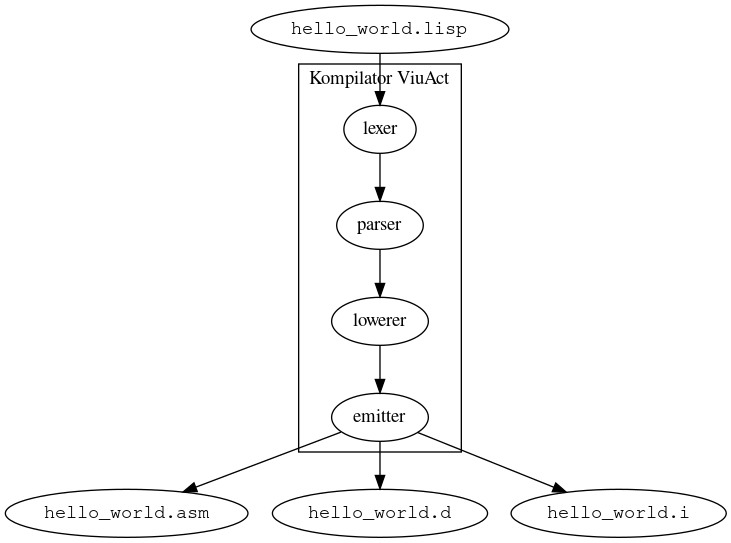
\includegraphics[width=10cm]{viuact-ogolny-schemat-kompilatora}
    \caption{Podział kompilatora na podsystemy}
    \label{ogolny_schemat_kompilatora_viuact}
\end{figure}

Każdy podsystem implementuje jedną z faz kompilacji:

\begin{enumerate}
    \item \textbf{lexer} dokonuje analizy leksykalnej wczytanego pliku źródłowego, dzieląc go na listę tokenów
    \item \textbf{parser} dokonuje analizy składniowej łącząc tokeny w grupy reprezentujące większe
        konstrukcje językowe
    \item \textbf{lowerer} mapuje grupy wyprodukowane przez \emph{parser} do odpowiednich funkcji
        \emph{emittera}; jest to dość banalny etap, ale upraszcza budowę kompilatora
    \item \textbf{emitter} tłumaczy konstrukcje językowe ViuAct na równoznaczne konstrukcje w języku
        assemblera Viua VM
\end{enumerate}

Różnica między podsystemami \emph{lowerer} i \emph{emitter} może być niejasna. Oba biorą udział w emisji
kodu wynikowego, ale \emph{lowerer} bezpośrednio zajmuje się tylko modułami i funkcjami, natomiast
\emph{emitter} implementuje emisję pojedynczych wyrażeń języka ViuAct -- przypisań \texttt{let}, konstrukcji
warunkowych \texttt{if}, wywołań funkcji, itd.

Proces kompilacji dokłaniej opisany jest w rozdziale \ref{opis_etapow_kompilacji}
(\nameref{opis_etapow_kompilacji}) na stronie \pageref{opis_etapow_kompilacji}.

\subsubsection{Program łączący -- \texttt{viuact-opt}}
\label{opis_linkera}

Program łączący (tzw. ,,\emph{linker}'') zajmuje się finalną fazą ,,kompilacji''.
Jest to stwierdzenie jednocześnie trafne i niepoprawne. Zazwyczaj jednak nie ma to znaczenia, ponieważ zarówno
linker jak i kompilator jest ukrywany przed programistą. Popularne ,,kompilatory'' jak np \emph{\texttt{g++}}
z GCC to tak naprawdę ,,drivery''; wywołanie polecenia \emph{\texttt{g++}} powoduje wywołanie zarówno
kompilatora (\emph{\texttt{cc1}}), assemblera (\emph{\texttt{as}}), jak i linkera (\emph{\texttt{ld}}) w taki
sposób aby na wyjściu uzyskać oczekiwany wynik, czyli na przykład plik wykonywalny w formacie
ELF \emph{\texttt{a.out}}.

W przypadku kompilatora ViuAct proces ten wygląda podobnie, ale nie jest aż tak zautomatyzowany.
Rolę ,,drivera'' pełni programista, który jest odpowiedzialny za wywołanie zarówno kompilatora jak i linkera.
Przykładowo:

\begin{lstlisting}
viuact-cc --mode exec ./hello_world.lisp
viuact-opt ./build/_default/hello_world.asm
\end{lstlisting}

Program łączący przeprowadzi proces asemblacji pliku podanego na wejściu, oraz dołączy do niego wszelkie
wymagane moduły. Zarówno asemblacja jak i łączenie będa przeprowadzone przez narzędzie dostarczane przez
platformę Viua VM -- \texttt{viuact-opt} zajmuje się jedynie wygenerowaniem odpowiednich poleceń dla tego
narzędzia.

Informacja o tym jakie moduły muszą zostać dołączone jest tworzona w oparciu o pliki zależności (opisane w
rozdziale \nameref{pliki_zaleznosci_modulow} na stronie \pageref{pliki_zaleznosci_modulow}).
Dla uproszczenia projektu program łączący nie zbiera informacji o zależnościach rekurencyjnie.

Po zebraniu informacji o zależnościach program łączący dokonuje asemblacji wszystkich modułów, od których
zależy kompilowany moduł główny. Następnie asembluje moduł główny i łączy wszystkie wyemitowane modułu
bytecode'u w gotowy plik wykonywalny.

\subsection{Przebieg procesu kompilacji}
\label{opis_etapow_kompilacji}

Ten rozdział zawiera dokładny opis procesu kompilacji, od momentu wczytania pliku z kodem źródłowym w języku
ViuAct do momentu wyemitowania kodu wynikowego w języku assemblera Viua VM. Kompilator jest wywoływany
poleceniem \texttt{viuact-cc} z opcją \texttt{-}\texttt{-mode} określającą czy kompilowany jest moduł wykonywalny
(\texttt{exec}) czy moduł biblioteki (\texttt{module}):

\begin{lstlisting}
viuact-cc --mode ( 'exec' | 'module' ) %*\emph{file.lisp}*)
\end{lstlisting}

\subsubsection{Wczytanie pliku źródłowego}

Kompilator wczytuje do pamięci cały plik źródłowy jako pojedynczy string.

\subsubsection{Analiza leksykalna}

Lexer patrzy na wczytany kod źródłowy i do pierwszego nieprzeanalizowanego znaku (czyli na początku analizy do
znaku na indeksie 0) próbuje przypasować wzorzec określający jaki token znajduje się na tej pozycji. Po udanym
przypasowaniu pozycja, która będzie rozpatrywana przez lexer jest przesuwana o tyle znaków ile wynosi długość
wygenerowanego tokenu i lexer rozpoczyna pracę od nowa. Ten proces trwa do momentu aż cały string wejściowy
nie zostanie przeanalizowany, albo odrzucony jako nieprawidłowy.

Algorytm przypasowania jest banalny. Lexer dysponuje listę wzorców (określonych przez wyrażenia regularne),
które określają jak wygląda każdy możliwy token w języku. Lexer po kolei próbuje przypasować każdy wzorzec z
listy i kończy na pierwszym trafieniu. Jeśli żaden wzorzec nie może zostać przypisany lexer odrzuca kod
źródłowy jako nieprawidłowy.

Wzorce są uszeregowane w taki sposób żeby nie była możliwa pomyłka i
na przykład przypasowanie początku nazwy zmiennej \texttt{letter} jako słowa kluczowego \texttt{let}.

\subsubsection{Analiza składniowa}
\label{opis_etapow_kompilacji_analiza_skladniowa}

Składnia języka została zaprojektowana w taki sposób aby analiza składniowa mogła być uproszczona do maksimum
i prosta w implementaji.

\paragraph{Grupowanie nawiasów}

W pierwszej fazie analizy składniowej tokeny grupowane są wegług nawiasów okrągłych, przy czym grupowanie jest
rekurencyjne (jeśli jakaś grupa zawiera podgrupę w nawiasach to zagnieżdżona grupa będzie widoczna jako
pojedynczy element w grupie zewnętrznej).
Dla przykładu:

\begin{lstlisting}
(let x (frobnicate 42))
\end{lstlisting}

będzie zgrupowane w następujący sposób:

\begin{lstlisting}
[ "let"; "x"; [ "frobnicate"; "42" ] ]
\end{lstlisting}

\paragraph{Grupowanie id}

Kolejnym etapem jest grupowanie id. Id jest nazwą składającą się z kilku członów, na przykład
\texttt{Std.Posix.Network.socket} składa się z 7 tokenów: trzech \emph{nazw modułów} (\texttt{Str},
\texttt{Posix}, i \texttt{Network}), trzech \emph{operatorów dostępu} (kropek), i jednej \emph{nazwy}
(\texttt{socket}).
Taka grupa zostanie na tym etapie zredukowana do pojedynczego elementu.

\paragraph{Oznczanie wyrażeń złożonych}

Wyrażenia złożone składają się z kilku wyrażeń (prostych bądź złożonych). Z uwagi na fakt, że formą pośrednią
wykorzystywaną na etapie grupowania są listy tokenów takie wyrażenie byłoby nieodróżnialne od listy
reprezentującej wywołanie funkcji. Dlatego na etapie analizy składniowej do list reprezentujących wyrażenia
złożone dodawany jest specjalny token-fantom. Dzięki temu zostaje zachowana właściwość umożliwiająca szybkie
klasyfikowanie grup. Dla przykładu:

\begin{lstlisting}
(let x { ... })
\end{lstlisting}

będzie zgrupowane w następujący sposób:

\begin{lstlisting}
[ "let"; "x"; [ Compound_expression_marker; ... ] ]
\end{lstlisting}

\paragraph{Klasyfikacja grup}

Ostatnim etapem analizy składniowej jest klasyfikacja grup. W większości przypadków do klasyfikacji listy
tokenów do grupy reprezentującej konkretną konstrukcję językową wystarczy spojrzeć na pierwszy token na
liście. W niektórych przypadkach algorytm musi się posiłkować długością listy.

Dla przykładu:

\begin{lstlisting}
[ "let"; "x";          ... ]        -> let-binding
[ "let"; "x"; [ ... ]; ... ]        -> function-definition
[ ... ]                             -> function-call
[ "actor"; ... ]                    -> actor-call
[ Compound_expression_marker; ... ] -> compound-call
\end{lstlisting}

Różnicą między definicją zmiennej (\texttt{let-binding}), a definicją funkcji (\texttt{function-definition})
jest długość listy - definicja zmiennej zawiera trzy elementy (słowo kluczowe \texttt{let}, nazwę, i
wyrażenie), a definicja funkcji cztery elementy (słowo kluczowe \texttt{let}, nazwę, listę parametrów
formalnych, i wyrażenie).

\subsubsection{Emisja modułów}

W następnej kolejności emitowane są wszystkie moduły zagnieżdżone w aktualnie kompilowanym module, przy czym
ten etap postępuje rekurencyjnie. Moduły zagnieżdżone musżą być wyemitowane przed modułem głównym, aby
kompilator miał dostęp do ich plików interfejsów i umożliwić ich importowanie.

\subsubsection{Analiza importu modułów}

Kolejnym krokiem jest analiza modułów importowanych przez aktualnie kompilowany moduł i wczytanie ich
interfejsów. Kompilator ładuje listy sygnatur funkcji i wyliczenia z każdego zaimportowanego modułu.

Jeśli kompilator nie może znaleźć pliku interfejsu danego modułu to kończy kompilację informując o błędzie.
Kompilator szuka plików interfejsów i modułów w ścieżkach podanych w zmiennej środowiskowej
\texttt{VIUAC\_LIBRARY\_PATH} (opisanej na stronie \pageref{viuact_manual_env_viuac_library_path}).

\subsubsection{Emisja kodu wynikowego}
\label{opis_etapow_kompilacji_emisja_kodu_wynikowego}

Na końcu następuje emisja kodu wynikowego w języku assemblera Viua VM. Ten etap jest wykonywany osobno dla
każdej funkcji zdefiniowanej w kompilowanym module.

\paragraph{Redukcja poziomu wyrażeń}

Najpierw następuje redukcja poziomu wyrażeń. Tym etapem zajmuje się \emph{lowerer}. Jest to mechaniczny proces
mapujący sklasyfikowane grupy reprezentujące konretne konstrukcje językowe do funkcji udostępnianych przez
\emph{emitter}, opakowanie wyniku w sposób jakiego wymagają zasady języka assemblera Viua VM, oraz
serializacja wyników do stringów.

\paragraph{Emisja instrukcji języka assemblera}

Emisja instrukcji języka assemblera jest wykonywana per-wyrażenie. Ten etap przeplata się z redukcją poziomu
wyrażeń i jest implementowany przez \emph{emitter}. \emph{Emitter} emituje sekwencje instrukcji języka
assemblera Viua VM odpowiadające zadanym konstrukcjom językowym ViuAct.

Dla przykładu \texttt{(let x 42)} zostanie wyemitowane jako pojedyncza instrukcja: \texttt{integer \%x local
42}.  Natomiast \texttt{(Some\_module.frobnicate 42)} zostanie wyemitowane jako sekwencja instrukcji:

\begin{lstlisting}
integer %3 local 42
frame %1 arguments
copy %0 arguments %3 local
call void Some_module::frobnicate/1
\end{lstlisting}

\subsubsection{Zapis pliku \texttt{.asm}}

Dla każdego wyemitowanego modułu kompilator zapisze plik \texttt{\emph{nazwa\_modulu}.asm} zawierający kod
wynikowy w języku assemblera Viua VM.

\subsubsection{Zapis pliku \texttt{.i}}

Dla każdego wyemitowanego modułu biblioteki kompilator zapisze plik \texttt{\emph{nazwa\_modulu}.i}
zawierający definicję interfejsu tego modułu. Pliki interfejsów są opisane w rozdziale
\nameref{pliki_interfejsow_modulow} na stronie \pageref{pliki_interfejsow_modulow}.

\subsubsection{Zapis pliku \texttt{.d}}

Dla każdego wyemitowanego modułu kompilator zapisze plik \texttt{\emph{nazwa\_modulu}.d}
zawierający definicję zależności tego modułu. Pliki zależności są opisane w rozdziale
\nameref{pliki_zaleznosci_modulow} na stronie \pageref{pliki_zaleznosci_modulow}.


\section{Projekt struktury}

\subsection{Wykorzystywane struktury danych}

Brak jest rozbudowanego diagramu klas, ponieważ program nie jest pisany w stylu obiektowym.
W programie istnieją dwie główne grupy struktur opisujące elementy języka -- typy tokenów i typy grup
(reprezentujących konstrukcje językowe), struktura reprezentująca adres rejestru (abstrakcyjny ,,slot'' na
wartości), struktura reprezentująca stan kompilowanego programu, oraz cztery struktury reprezentujące
niskopoziomowe abstrakcje linii programu w języku assemblera -- konstruktor, przeniesienie, wywołanie, i
,,\emph{verbatim}''.

\begin{quote}
    Listingi przedstawiające wykorzystywane struktury danych jest podany w języku OCaml.
    Kompilator jest napisany w języku Python, który nie pozwala na tak łatwe i czytelne definiowanie
    nowych struktur danych -- stąd decyzja o użyciu innego języka w pracy.

    Zachowane zostały typy danych, nazwy pól i całych struktur. OCaml pozwala na duże bardziej
    przejrzyste i czytelne opisanie typów danych poszczególnych pól niż Python, co ma dużą
    wartość dokumentacyjną.
\end{quote}

\subsubsection{Tokeny}
\label{diagram_klas_tokeny}

Każdy typ tokenu jest reprezentowany przez osobną strukturę. Tokeny, oprócz swojego typu mają atrybuty
określające ich lokalizację w pliku (wiersz i kolumna), oraz pole z leksemem. Typy tokenów wymagane do
reprezentacji języka ViuAct są opisane w specyfikacji języka.

Definicje struktur reprezentujących tokeny są zawarte w pliku \texttt{viuact/token\_types.py}.

\subsubsection{Grupy}
\label{diagram_klas_grupy}

Każda konstrukcja językowa jest reprezentowana przez osobną strukturę. Konstrukcje wymagane do reprezentacji
języka ViuAct są opisane w specyfikacji języka.

Definicje struktur reprezentujących grupy są zawarte w pliku \texttt{viuact/group\_types.py}.

\subsubsection{Slot}
\label{diagram_klas_slot}

\begin{lstlisting}
enum Register_set =
    | Local
    | Parameters
    | Arguments
    | Closure_local

type Slot = {
    name         : string ;
    index        : int ;
    register_set : register_set ;
}
\end{lstlisting}

Struktura \texttt{Slot} reprezentuje adres rejestru. Z punktu widzenia języka ViuAct istotne jest pole
\texttt{name} (określające nazwę slotu jaką posługuje się programista); z punktu widzenia emitera kodu istotne
są pola \texttt{index} i \texttt{register\_set} określające adres rejestru jakim posługuje się Viua VM.

\subsubsection{Stan programu}
\label{diagram_klas_stan_programu}

Stan programu (struktura \texttt{State}) zawiera pola śledzące ilość zaalokowanych rejestrów, widoczne
funkcje, a w przypadkach śledzenia stanu funkcji zagnieżdżonej -- także wykorzystywane sloty z otaczającego
zakresu leksykalnego.

\subsubsection{Konstruktor}
\label{diagram_klas_konstruktor}

\begin{lstlisting}
type Ctor = {
    of_type : string ;
    slot    : Slot ;
    value   : string ;
}
\end{lstlisting}

Konstruktor reprezentuje instrukcję bezpośrednio tworzącą wartość w rejestrze. Przykładowo, aby wyemitować
instrukcję \texttt{integer \%1 local 42} utworzony zostanie:

\begin{lstlisting}
{
    of_type = "integer" ;
    slot = { name = "x"; index = 1 ; Register_set.Local } ;
    value = "42"
}
\end{lstlisting}

\subsubsection{Przeniesienie}
\label{diagram_klas_przeniesienie}

\begin{lstlisting}
enum Move_kind =
    | Move
    | Copy

type Move = {
    kind   : Move_kind ;
    source : Slot ;
    dest   : Slot option ;
}
\end{lstlisting}

Przeniesienie opisuje przesunięcie (instrukcja \emph{\texttt{move}}) lub kopię wartości (instrukcja
\emph{\texttt{copy}}). Slot docelowy nie musi być obecny - np. wtedy wartość jest przenoszona do slotu
\texttt{void}.

\subsubsection{Wywołanie}
\label{diagram_klas_wywolanie}

\begin{lstlisting}
enum Call_kind =
    | Synchronous
    | Actor
    | Tail
    | Deferred

type Call = {
    kind : Call_kind ;
    slot : Slot option ;
    to   : string ;
}
\end{lstlisting}

Wywołanie opisuje wywołanie funkcji w każdy sposób dostępny w języku ViuAct: zwykłe wywołanie funkcji,
wywołanie tworzące aktora, wywołąnie \emph{tail call}, i wywołanie ''odroczone''.

Typy wywołań opisane są w specyfikacji języka.

\subsubsection{Linia ''\emph{verbatim}''}
\label{diagram_klas_linia_verbatim}

\begin{lstlisting}
type Verbatim = {
    text : string ;
}
\end{lstlisting}

Linia \emph{verbatim} opisuje dowolną linię języka assemblera (m.in. dyrektywy \texttt{.import:} czy
\texttt{.function:}).

\emph{Emitter} (rozdział \ref{opis_etapow_kompilacji_emisja_kodu_wynikowego} na stronie
\pageref{opis_etapow_kompilacji_emisja_kodu_wynikowego}) większość instrukcji tworzy za pomocą linii
\emph{verbatim}. Jest to zabieg o tyle ''brzydki'' co efektywny; na etapie prototypowania bardzo szybko
można w ten sposób wyemitować spory zakres instrukcji bez potrzeby projektowania struktury dla każdego typu
instrukcji.

\section{Decyzje projektowe}

\subsection{Środowisko docelowe}

Środowiskiem docelowym, na którym będą uruchamiane programy napisane w języku \ViuAct jest maszyna wirtualna
Viua VM. Środowisko docelowa musi spełniać wymagania jakie ma Viua VM (m.in. musi to być system zgodny ze
standardem POSIX).

\subsection{Środowisko implementacji}

Środowiskiem implmentacji jest Linux z dostępnymi standardowymi narzędziami GNU, językiem Python 3, i
umożliwiającym uruchomienie assemblera dostarczanego przez Viua VM.

\subsection{Priorytety implementacyjne}

Maksymalizacja prostoty budowy kompilatora i języka.
Marginalizacja obsługi błędów w kompilatorze z uwagi na brak czasu.
Marginalizacja optymalizacji z uwagi na brak czasu.

\section{Projekt algorytmów i przyjętych protokołów}

Dyskusja na temat algorytmów i sposobu implementacji jest częściowo przeprowadzona w rozdziale
\ref{opis_etapow_kompilacji} na stronie \pageref{opis_etapow_kompilacji}, szczególnie w rozdziale
\ref{opis_etapow_kompilacji_analiza_skladniowa}.

\section{Projekt rozwiązań sprzętowych}

Brak w tym projekcie. Jest on wyłącznie softwareowy.

\section{Projekt interfejsu}

\subsection{Interfejs użytkownika}

Interfejs użytkownika opisany jest w osobnym dokumencie -- podręczniku użytkownika kompilatora ViuAct (plik
''viuact-manual.pdf'').

\subsubsection{Założenia konstrukcji interfejsu}

\subsection{Interfejs kompilatora}

Kompilator składa się z dwóch programów: \texttt{viuact-cc} (kompilatora właściwego) i \texttt{viuact-opt}
(programu łączącego). Programy te są konfigurowane za pomocą zmiennych środowiskowych, które kontrolują poziom
''głośności'' logów, położenie assemblera Viua VM, a także włączają bądź wyłączają serializację formy
pośredniej.

Interfejs kompilatora opisany jest w osobnym dokumencie.

\subsection{Interfejs języka}

Interfejsem języka jest jego składnia.
Jest ona opisana w specyfikacji języka.

\subsection{Inne interfejsy}

\subsubsection{Pliki interfejsów modułów (\texttt{.i})}
\label{pliki_interfejsow_modulow}

Pliki interfejsów modułów wyliczają funkcje eksportowane przez dany moduł, oraz prezentują metadane wymagane
do połączenia plików w sposób, który będzie mógł działać na Viua VM. Pliki interfejsu dla modułów ''własnych''
nie różnią się zasadniczą strukturą od plików interfejsu dla modułów ''obcych'', ale pliki interfejsu dla
modułów ''obcych'' muszą być uzupełnione o kilka dodatkowych pól. Jest to dokładniej opisane w rozdziale
\ref{pliki_interfejsow_modulow_obcych} na stronie \pageref{pliki_interfejsow_modulow_obcych}.

Pliki interfejsów są zapisywane w formacie JSON.

\paragraph{Plik interfejsu dla modułów ''własnych''}

Moduły ''własne'' języka ViuAct to moduły napisane w języku ViuAct.

\begin{lstlisting}
{
    "foreign": false,
    "real_name": "A_module",
    "fns": [
        {
            "arity": 1,
            "name": "f",
            "real_name": "A_module::f",
            "from_module": "A_module"
        }
    ]
}
\end{lstlisting}

Atrybut \texttt{foreign} określa czy moduł jest ''obcy'' (\texttt{true}) czy ''własny'' (\texttt{false}).
Atrybut \texttt{real\_name} określa nazwę modułu tak jak będzie prezentowana na poziomie bytecode'u.
Atrybut \texttt{fns} jest listą funkcji, które są przez dany moduł eksportowane.

W elementach listy \texttt{fns} atrybuty mają następujące znaczenie:

\begin{enumerate}
    \item \texttt{arity} określa ''moc'' funkcji
    \item \texttt{name} określa nazwę funkcji widoczną z poziomu języka ViuAct
    \item \texttt{real\_name} określa pełną nazwę funkcji widoczną z poziomu bytecode'u
    \item \texttt{from\_module} określa pełną nazwę modułu, z którego pochodzi dana funkcja
\end{enumerate}

\paragraph{Plik interfejsu dla modułów ''obcych''}
\label{pliki_interfejsow_modulow_obcych}

Moduły ''obce'' języka ViuAct to moduły napisane w języku assemblera Viua VM lub w C++.

\begin{lstlisting}
{
    "foreign": true,
    "real_name": "std::posix::network",
    "fns": [
        {
            "arity": 0,
            "name": "socket",
            "real_name": "Std::Posix::Network::socket",
            "bytecode_name": "std::posix::network::socket",
            "from_module": "Std::Posix::Network"
        }
    ]
}
\end{lstlisting}

Różnicą w stosunku do plików interfejsu dla modułow ''własnych'' jest dodatkowy atrybut w deklaracji
eksportowanej funkcji -- \texttt{bytecode\_name} określający nazwę funkcji na poziomie bytecode'u. Nazwa ta
nie musi pokrywać się z nazwą w atrybucie \texttt{real\_name}, który określa pełną nazwę funkcji widoczną na
poziomie języka ViuAct.

Dwa atrybuty są potrzebne ponieważ na tym poziomie następuje łączenie dwóch ''światów''; języka ViuAct, który
narzuca reguły tego jak muszą wyglądać nazwy modułów i funkcji, oraz języka assemblera Viua VM, który takich
reguł nie narzuca. Dla modułów ''własnych'' atrybuty \texttt{bytecode\_name} jest zbędny ponieważ dla nich
nazwa widoczna na poziomie ViuAct i języka assemblera Viua VM jest taka sama.

\subsubsection{Pliki zależności modułów (\texttt{.d})}
\label{pliki_zaleznosci_modulow}

Pliki zależności są kodowane w formacie JSON.

\begin{lstlisting}
{
    "imports": [
        {
            "module_name": "Std::Random",
            "real_name": "std::random",
            "foreign": true
        }
    ]
}
\end{lstlisting}

Atrybut \texttt{imports} przechowuje listę modułów importowanych przez moduł, którego zależności definiuje
dany plik (co jest określane na podstawie nazwy pliku).

W elementach listy \texttt{imports} atrybuty mają następujące znaczenie:

\begin{enumerate}
    \item \texttt{module\_name} określa pełną nazwę modułu z punktu widzenia języka ViuAct
    \item \texttt{real\_name} określa pełną nazwę modułu widoczną z poziomu bytecode'u
    \item \texttt{foreign} określa czy moduł jest ''własny'' (\texttt{false}) czy ''obcy'' (\texttt{true})
\end{enumerate}

\section{Projekt bazy danych}

Brak bazy danych jako takiej w projekcie.
Dane przetwarzane przez kompilator są trzymane w plikach, których struktura opisana jest w rozdziałach
\ref{pliki_interfejsow_modulow} na stronie \pageref{pliki_interfejsow_modulow} i
\ref{pliki_zaleznosci_modulow} na stronie \pageref{pliki_zaleznosci_modulow}.

\section{Opis implementacji}

Implementacja kompilatora jest bardzo prosta, jak na standardy tego typu projektów.
Rysunek \ref{basic_compiler_flow} na stronie \pageref{basic_compiler_flow} bardzo dobrze oddaje strukturę
kompilatora dostarczonego jako wynik tej pracy.

\paragraph*{Analiza leksykalna i składniowa}
W fazie przygotowania tekstu programu ''do obróbki'' najpierw przeprowadzana jest analiza leksykalna (podział
tekstu na tokeny), później analiza składniowa -- która w dużej mierze polega na uporządkowaniu ''płaskiej''
listy tokenów w grupy ograniczone nawiasami. Algorytm dokonujący analizy składniowej jest trywialny:

\begin{enumerate}
    \item utwórz pustą listę przetworzoną
    \item rozważ token pierwszy nieprzenalizowany token
    \item jeśli ten token to \texttt{(} lub \texttt{\{}, rozpocznij rekurencyjnie przetwarzanie strumienia
        tokenów od następnego tokenu, a wynik analizy dodaj jako pojedynczy element do listy przetworzonej
    \item w innym przypadku dodaj token do listy przetworzonej
    \item jeśli na strumień tokenów jest pusty, zakończ algorytm
    \item w innym przypadku kontynuuj od punktu 2.
\end{enumerate}

Na pierwszy rzut oka widać, że ten algorytm nie analizuje wiele -- jego jedynym zadaniem jest pogrupowanie
płaskiego, jednowymiarowego strumienia tokenów w grupy reprezentujące konkretne konstrukcje językowe. Prostota
algorytmu sprawia, że jest on też bardzo szybki w działaniu.

Faktycznie, na tym etapie łączone są również rozbudowane identyfikatory (np. \texttt{foo.bar.baz}), ale nie
wpływa to znacząco na skomplikowanie kodu.

\paragraph*{Klasyfikacja grup}
Po tym etapie ''wstępnej'' analizy następuje klasyfikacja grup. W tym przypadku algorytm również jest bardzo
prosty. Klasyfikator rekurencyjnie sprawdza wszystkie listy i nadaje im typ oznaczający jaką konstrukcję
językową reprezentują. W tym celu musi jedynie sprawdzić typ pierwszego tokenu, i ewentualnie (w przypadku
dowiązań \emph{\texttt{let}} i definicji funkcji) długość listy.

Wykorzystanie algorytmu o tak niskim poziomie złożoności jest możliwe dzięki uważnemu zaprojektowaniu składni
języka. Każda konstrukcja językowa jest grupowana nawiasami -- klamrowymi bądź okrągłymi -- lub ma stałe
miejsce w grupie. Poniżej, dla przykładu, zaprezentowane są wzorce odpowiadające wybranym konstrukcjom
językowym:
\begin{lstlisting}
(let   %*\emph{name}*) %*\emph{expression}*))
(if    %*\emph{condition-expr}*) %*\emph{true-expr}*) %*\emph{false-expr}*))
(try   %*\emph{guarded-expr}*) ...)
(actor %*\emph{id}*) %*\emph{expr}*)*)
(+     %*\emph{lhs-expr}*) %*\emph{rhs-expr}*))
\end{lstlisting}

Jeśli całość oprócz pierwszego tokenu zostanie ''ukryta'' to dalej oczywistym jest z jaką konstrukcją mamy do
czynienia:
\begin{lstlisting}
(let   ...)
(if    ...)
(try   ...)
(actor ...)
(+     ...)
\end{lstlisting}

Wykorzystanie notacji polskiej (notacji prefiksowej) i takie zaprojektowanie składni, że każda konstrukcja ma
stałą ''szerokość'' pozwala na zastosowanie chwytu ''\emph{pierwszy token decyduje}''. Sprawia to też, że
język ma rozpoznawalne tempo i styl, a konsekwencja układu nadaje mu elegancji.


\section{Testowanie}

Testy kompilatora.

\subsection{Zestaw przypadków testowych}

Jeden testowy program na każdą funkcjonalność języka.
Kilka większych testowych programów sprawdzających integrację języka, np. wielomodułowych, wykorzystujących
moduły obce.

\subsection{Wykonanie testów}

Opis tego jak wygląda uruchomienie testów, w jaki sposób został zbudowany framework, itp.

\subsection{Trudności w testowaniu}

Niedeterminizm wynikający z równoległego działania aktorów stwarza problemy w testach. Trzeba uciekać się do
"sztuczek", np. sortowanie wyników programu testowego.

\section{Instrukcja użytkownika kompilatora języka Viuact}
\label{viuact_manual}

Tradycja nakazuje, aby pierwszym programem jaki pisze się w nowym języku był program, który wypisze na ekran
napis ,,\emph{Hello World!}''. W ViuAct ten program wygląda następująco:

\begin{lstlisting}
(let main () {
    (print "Hello World!")
    0
})
\end{lstlisting}

Aby skopilować ten program, należy wykonać w konsoli następujące polecenia:

\begin{lstlisting}
$ viuact-cc --mode exec ./hello_world.lisp
$ viuact-opt ./build/_default/hello_world.asm
\end{lstlisting}

Kod wykonywalny (\emph{bytecode} wykonywalny przez Viua VM) będzie umieszczony w pliku
\texttt{hello\_world.bc} w katalogu \texttt{./build/\_default}.
Aby go uruchomić należy użyć jądra Viua VM:

\begin{lstlisting}
$ viua-vm ./build/_default/hello_world.bc
%*\emph{Hello World!}*)
$
\end{lstlisting}

Nazwy plików pośrednich są wywodzone z nazwy pliku źródłowego:

\begin{description}
    \item[\texttt{\emph{example}.lisp}] plik z kodem źródłowym w języku ViuAct
    \item[\texttt{\emph{example}.asm}] plik wynikowy kompilatora, z kodem źródłowym w języku assemblera Viua
        VM
    \item[\texttt{\emph{example}.bc}] plik wynikowy assemblera Viua VM, zawierający wykonywalny bytecode
\end{description}

Pliki \texttt{.asm} i \texttt{.bc} są umieszczane w katalogu \texttt{./build/\_default}.

\subsection{Opcje kompilatora}

Jedyną opcją kompilatora jest \texttt{--mode}, która przyjmuje dwie możliwe wartości:

\begin{description}
    \item[\texttt{exec}] jeśli plik źródłowy definiuje moduł wykonywalny
    \item[\texttt{module}] jeśli plik źródłowy definiuje moduł biblioteczny
\end{description}

\subsection{Zmienne środowiskowe}

Zachowanie kompilatora można częściowo zmodyfikować ustawiając zmienne środowiskowe.

\subsubsection{\texttt{DEFAULT\_OUTPUT\_DIRECTORY}}

Kontroluje katalog, w którym kompilator składuje pliki wynikowe. Domyślnie pliki wynikowe są składowane w
katalogu \texttt{./build/\_default}.

\subsubsection{\texttt{VIUAC\_LIBRARY\_PATH}}

Jak \texttt{LD\_LIBRARY\_PATH}.

\subsubsection{\texttt{VIUA\_ASM\_PATH}}

Kontroluje ścieżkę do assemblera Viua VM.

\subsubsection{\texttt{VIUAC\_VERBOSE}}

Wartość \texttt{true} powoduje wyświetlenie komunikatów podczas kompilacji.

\subsubsection{\texttt{VIUAC\_DEBUGGING}}

Wartość \texttt{true} włącza komunikaty debugowania.

\subsubsection{\texttt{VIUAC\_INFO}}

Wartość \texttt{true} włącza dodatkowe komunikaty informacyjne.

\subsubsection{\texttt{VIUAC\_DUMP\_INTERMEDIATE}}

Wartość \texttt{tokens} powoduje zrzut strumienia tokenów do pliku \texttt{\emph{example}.tokens}.
Wartość \texttt{exprs} powoduje zrzut drzewa składni do pliku \texttt{\emph{example}.expressions}.
Można podać obie wartości, oddzielone przecinkiem.

\subsection{Opcje programu łączącego}

